\documentclass[a4paper]{article}
% Kodowanie latain 2
%\usepackage[latin2]{inputenc}
\usepackage[T1]{fontenc}
% Można też użyć UTF-8
\usepackage[utf8]{inputenc}
\usepackage[parfill]{parskip}

% Język
\usepackage[polish]{babel}
% \usepackage[english]{babel}

% Rózne przydatne paczki:
% - znaczki matematyczne
\usepackage{amsmath, amsfonts}

% - szersza strona
\usepackage[nofoot,hdivide={2cm,*,2cm},vdivide={2cm,*,2cm}]{geometry}

% - obrazki
\usepackage{graphics}
\usepackage{graphicx}

\usepackage{hyperref}

% - brak numerów stron
\pagestyle{empty}

% dane autora
\author{Wiktor Ogrodnik}
\title{Program Wykresy - instrukcja obsługi}
\date{\today}
\usepackage{enumitem}

% początek dokumentu
\begin{document}
\maketitle

\section{Opis programu}
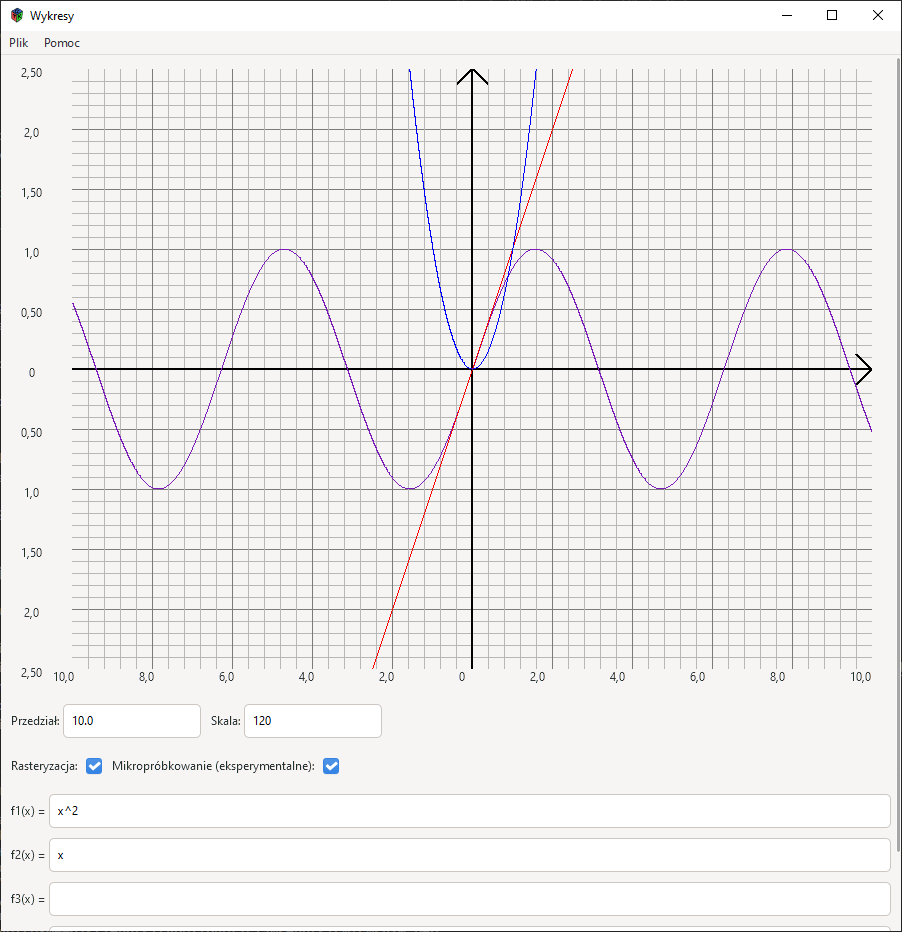
\includegraphics[scale = 0.5]{img2.png}

Program wykresy służy do rysowania wykresów jednej zmiennej w zadanym przedziale. Wykres rysuje się w górnej części programu po naciśnięciu przycisku wprowadź. Program posiada zaawansowany interpreter obsługujący operatory matematyczne, funkcje takie jak sinus czy logarytm, kolejność wykonywania działań, dowolną ilość nawiasów oraz stałe matematyczne. Moduł wyświetlający wykres na ekranie ma zaimplementowany system prostej rasteryzacji, dzięki czemu nawet wykresy skomplikowanych funkcji prezentują się w przystępny sposób. Wspierane systemy operacyjne to Windows 10 i Linux.

\subsection{Technologie}
Technologie użyte do stworzenia programu to:
\begin{itemize}
    \item Język C11 (GCC 10.2),
    \item Biblioteka GTK+ 3.24,
    \item Program make,
    \item Visual Studio Code.
\end{itemize}

\section{Kompilacja ze źródła i uruchamianie}

\subsection{Windows}
\begin{itemize}
    \item pobrać i zainstalować MSYS2, zgodnie z zaleceniami ze strony \url{https://www.msys2.org/};
    \item pobrać i zainstalować bibliotekę GTK (GTK+ 3.24) zgodnie z instruckją na stronie \url{https://www.gtk.org/docs/installations/windows/};
    \item jeżeli nie są zainstalowne, przez menedżer pakietów MSYS2 pobrać kompilator mingw i program make;
    \item poprzez konsolę MSYS2 MinGW 64-bit (lub 32-bit) odnaleźć folder z kodem źródłowym i wpisać polecenie 'make';
    \item uruchomić program poleceniem ./wykresy.exe.
\end{itemize}

\subsection{Linux}
\begin{itemize}
    \item poprzez wbudowany w dystrybucje menedżer pakietów pobrać i zainstalować pakiet 'libgtk-3-dev' wraz z pakietmai zależnymi;
    \item jeżeli nie są zainstalowane, przez wbudowany w dytrybucje menedżer pakietów pobrać kompilator gcc i program make;
    \item w terminalu odnaleźć folder z kodem źródłowym i wpisać polecenie 'make';
    \item uruchomić program poleceniem ./wykresy.
\end{itemize}

\section{Równania matematyczne}

W tej sekcji opiszę jakie możliwości daje intepreter poleceń matematycznych wbudowany w program i jak konstruować zapytania. W programie można wpisać na raz 4 równania, które będą wyświetlane jednocześnie na wykresie.

\subsection{Składnia}
\begin{itemize}
    \item liczby
    \item funkcje
    \item stałe
    \item zmienna
    \item nawiasy
    \item operatory binarne
\end{itemize}

\subsubsection{Liczba}

Liczba to stała zapisana za pomocą cyfr oraz kropki i przecinka ({0, 1, 2, 3, 4, 5, 6, 7, 8, 9, 0,, ,.}). Liczby to np. 10, 2,5, 10.5, 0, 11, 123, itd.
Przed liczbą może znajodwać się '+' lub '-' oznaczający znak liczby, np: +10, -0.5.

\subsubsection{Funkcje}

Funkcje składają się z nazwy, nawiasów okrągłych oraz przyjmują jeden argument. Np.: sin(<wyrażenie>), log(<wyrażenie>), itd.

W programie dostępne są następujące funkcje:
\begin{itemize}
    \item sin(x)
    \item cos(x)
    \item tan(x) - inna forma: tg(x)
    \item cot(x) - inna forma: ctg(x)
    \item ln(x) - logarym naturalny, również log(x)
    \item log2(x) - logarytm dwójkowy
    \item log10(x) - logarytm dziesiątkowy
    \item sqrt(x) - pierwiastek kwadratowy
    \item abs(x) - wartość bezwzględna
    \item sinh(x) - sinus hiperboliczny
    \item cosh(x) - cosinus hiperboliczny
    \item tanh(x) - tangens hiperboliczny, również tgh(x)
    \item floor(x) - część całkowita, tak zwana podłoga
    \item ceil(x) - część całkowita (zaokrąglenie w górę), tak zwany sufit
    \item asin(x) - arcus sinus, również arcsin(x)
    \item acos(x) - arcus cosinus, również arccos(x)
    \item atan(x) - arcus tangens, również arctan(x) i arctg(x)
    \item exp(x) - funkcja ekspotencjalna ($e^x$)
\end{itemize}


\subsubsection{Stałe}

W programie zdefiniowane są 3 specjalne stałe, można je wpisywać tak samo jak liczby:
\begin{itemize}
    \item e - $e$
    \item pi - $\pi$
    \item phi - $\phi$
\end{itemize}

\subsubsection{Zmienna}

Jako, że program rysuje funkcje jednej zmiennej, to dostepna jest tylko jedna zmienna - 'x'. Intepreter pod zmienną x podstawia odpowiednią wartość liczbową, w zależności od części wykresu, która jest rysowana.

Uwaga! Użycie innej litery niż x jako zmiennej nie zadziała!

\subsubsection{Nawiasy}

Dostepne są 4 rodzaje nawiasów:
\begin{itemize}
    \item Nawiasy okrągłe '()' - zwykłe nawiasy bez specjalnych funkcji, wyrażenie w tych nawiasach wykonywane jest w pierwszej kolejności. Dzięki nim można wpływać na kolejność wykonywania działań.
    \item Nawiasy typu '||' - posiadają funkcje nawiasów okrągłych, a dodatkowo obliczają wartość bezwzględną. Równoważne byłoby użycie funkcji abs(<wyrażenie>).
    \item Nawiasy kwadratowe '[]' - oprócz tego, że wyrażenie w nawiasach wykonywane jest w pierwszej kolejności, to zwaracana jest część całkowita tego wyrażenia. Równoważne byłoby użycie funkcji floor(<wyrażenie>).
    \item Nawiasy klamrowe '\{\}' - wyrażenie w nawiasach wykonywane jest w pierwszej kolejności i zwracana jest część ułamkowa wyrażenia.
\end{itemize}

\subsubsection{Operatory binarne}

W programie jest 5 operatorów binarnych, przyjmujących dwa argumenty, jeden z prawej, drugi z lewej strony operatory. 

Dostepne operatory:
\begin{itemize}
    \item x+y - dodawanie $x+y$
    \item x-y - odejmowanie $x-y$
    \item x*y - mnożenie $x*y$
    \item x/y - dzielenie $x/y$
    \item x\^{}y - potęgowanie $x^y$ 
\end{itemize}

Operatory mają różne priorytety. Najpierw wykonywane jest potęgowanie, potem mnożenie i dzielenie, a na końcu dodawanie i odejmowanie.

Jeżeli operatory mają ten sam priorytet wykonywane są od lewej do prawej, wyjątkiem jest potęgowanie, które wykonuje się w drugą stronę.

Polecenie 'x\^{}y\^{}z' jest interpretowanie jako $x^{y^z}$. 
Ale 'x\^{}y\^{}z*a' jest interpretowanie jako $x^{y^z} \times a$. Dlatego zalecane jest stosowanie nawiasów, żeby uniknąć nieporozumień.

Czasem niewymagane jest pisanie znaku mnożenia. Np. '2x' intepretowane jest jako '2 * x', 2(x + 3) interpretowane jest jako 2*(x+3).

Jako x i y można podstawić zmienną, stałe, liczby, wyrażenie w nawiasach lub funkcje.

\subsection{Semantyka}

Poprawne wyrażenia matematyczne w programie:
\begin{itemize}
    \item Każda liczba, stała i zmienna jest poprawnym wyrażeniem
    \item <wyrażenie> <op> <wyrażenie> jest poprawnym wyrażeniem, gdzie <op> to '+', '-', '*', '/' lub '\^{}'
    \item nazwafunkcji(<wyrażenie>) jest poprawnym wyrażeniem
    \item (<wyrażenie>) jest poprawnym wyrażeniem (gdzie '()' to dowolne nawiasy)
\end{itemize}

Wszystkie wyrażenia matematyczne można skonstruować według powyższej zasady.

W zapytaniach można używać dowolnej liczby spacji lub nie używać jej wcale, wyjątkiem są spacje wewnątrz liczby, nazwy funkcji lub stałej, które są niedozwolone.

\subsection{Przykłady równań}

W tym dziale zawarłem konkretne przykłady funkcji jednej zmiennej i wyjaśnienie jak będą zinterpretowane przez program.

\begin{itemize}
    \item 2 + x => $2 + x$
    \item sin(x\^{}2/10+5\^{}2\^{}(x)) => sin$(\frac{x^2}{10} + 5^{2^x})$
    \item cos(x)\^{}2 - 10/x*2 => $cos^2 (x) - \frac{10}{x} * 2$
    \item cos(x)\^{}2 - 10/(x*2) => $cos^2 (x) - \frac{10}{2x}$
    \item 10 + (2 + 3) - floor(x\^{}2)\^{}2 => $10 + (2 + 3) - floor^2(x^2)$
\end{itemize}

\section{Ustawienia}
W programie znajduje się kilka ustawień, którymi można zarządzać jak funkcje mają być wyświetlane na wykresie.
\subsection{Przedział}
Pole tekstowe przedział przyjmuje jedną liczbę (może być to liczba całkowita lub liczba ze skończonym rozwinięciem dziesiętnym). Po wpisaniu 10.0 funkcja będzie rysowana na przedziale od -10 do 10.
\subsection{Skala}
Pole tekstowe skala przyjmuje jedną liczbę (może być to liczba całkowita lub liczba ze skończonym rozwinięciem dziesiętnym). Skala odpowiada za przeciwdziedzinę na jakiej rysowana będzie funkcja. Przy skali 1.0 najmniejsza wartość jaką można zobaczyć to f(x) = -300, a nazjwiększa +300, przy skali 2.0 przedział to (-150, 150), przy domyślnej skali 30.0 przedział to (-10, 10).
\subsection{Rasteryzacja i Mikropróbkowanie}

Rasteryzacja odpowiada za łączenie kropek na wykresie, tak żeby wyświetlany wykres był ciągłą linią. Opcja ta zalecana jest gdy wykres szybko rośnie lub maleje, bez rasteryzacji ciężko byłoby zaobserwować przebieg funkcji. 
Uwaga! Rasteryzacja w punktach nieciągłości może zachowywać się nieprzewidywalnie, np. dla wyrażenia 'floor(x)' funkcjonalność będzie rysowała pionowe linie w punktach f(k), gdzie k jest liczbą całkowitą, co nie powinno mieć miejsca.
Rasteryzacja ma mały wpływ na wydajność i jest włączona domyślnie.

Mikropróbkowanie działa tylko przy włączonej rasteryzacji. Funkcjonalność wykonuje dodatkowe testy w punktach nieciągłości i decyduje czy rysować linie łączącą kropki czy nie. Funkcjonalność jest eksperymentalna, ale powinna lepiej odzwierciedlać wykresy skomplikowanych funkcji.
Mikropróbkowanie ma duży wpływ na wydajność i jest domyślnie wyłączone.

\section{Przewodnik po kodzie programu}

W programie znajdują się następujące moduły
\begin{itemize}
    \item Intepreter poleceń matematycznych w plikach eval.h i eval.c,
    \item Moduł wyświetlający wykres w plikach draw.h i draw.c,
    \item Moduł rysujący interfejs w plikach ui.h i ui.c,
    \item Moduł zawierający konwertery pomiędzy typami w C w plikach convert.h i convert.c,
    \item Używane struktury zdefiniowane są w pliku types.h.
\end{itemize}

Wyjaśnienie działania poszczególnych funkcji jest wyjaśnione w komentarzach wewnątrz programu.

\section{Dalszy rozwój}

Po zakończeniu projektu planuję dalsze prace nad programem. Oprócz rozwoju samego kodu, gdzie planuję migrację do GTK 4 oraz wykorzystywanie XML i CSS przy rysowaniu interfejsu, zaplanowane są również następujące funkcjonalności:

\begin{itemize}
    \item Wsparcie dla funkcji o kilku arguemntach, np. logarytm dowolnej podstawy;
    \item Rysowanie wykresu pochodnej;
    \item Zapisywanie wykresu do pliku .bmp;
    \item Zapis i odczyt funkcji z pliku tekstowego;
    \item Parametry uruchamiania programu z konsoli;
    \item Menu ustawień i "Co nowego";
    \item Konfiguracja własnych stałych matematycznych;
    \item Moduł automatycznych aktualizacji.
\end{itemize}

\section{Licencjonowanie}

Program wykresy będzie darmowym oprogramowaniem open-source na licencji MIT. Po oddaniu projektu kod zostanie otwarty i będzie dostepny w publicznym repozytorium na GitHubie.

\end{document}